%%%%%%%%%%%%%%%%%%%%%%%%%%%%%%%%%%%%%%%%%
% Journal Article
% LaTeX Template
% Version 1.3 (9/9/13)
%
% This template has been downloaded from:
% http://www.LaTeXTemplates.com
%
% Original author:
% Frits Wenneker (http://www.howtotex.com)
%
% License:
% CC BY-NC-SA 3.0 (http://creativecommons.org/licenses/by-nc-sa/3.0/)
%
%%%%%%%%%%%%%%%%%%%%%%%%%%%%%%%%%%%%%%%%%

%----------------------------------------------------------------------------------------
%	PACKAGES AND OTHER DOCUMENT CONFIGURATIONS
%----------------------------------------------------------------------------------------

\documentclass[twoside]{article}

\usepackage{lipsum} % Package to generate dummy text throughout this template

\usepackage[sc]{mathpazo} % Use the Palatino font
\usepackage[T1]{fontenc} % Use 8-bit encoding that has 256 glyphs
\linespread{1.05} % Line spacing - Palatino needs more space between lines
\usepackage{microtype} % Slightly tweak font spacing for aesthetics

\usepackage[hmarginratio=1:1,top=30mm,columnsep=20pt, hmargin = 2 cm]{geometry} % Document margins
\usepackage{multicol} % Used for the two-column layout of the document
\usepackage[hang, small,labelfont=bf,up,textfont=it,up]{caption} % Custom captions under/above floats in tables or figures
\usepackage{booktabs} % Horizontal rules in tables
\usepackage{float} % Required for tables and figures in the multi-column environment - they need to be placed in specific locations with the [H] (e.g. \begin{table}[H])
\usepackage{hyperref} % For hyperlinks in the PDF

\usepackage{lettrine} % The lettrine is the first enlarged letter at the beginning of the text
\usepackage{paralist} % Used for the compactitem environment which makes bullet points with less space between them

\usepackage{abstract} % Allows abstract customization
\renewcommand{\abstractnamefont}{\normalfont\bfseries} % Set the "Abstract" text to bold
\renewcommand{\abstracttextfont}{\normalfont\small\itshape} % Set the abstract itself to small italic text

\usepackage{titlesec} % Allows customization of titles
\renewcommand\thesection{\Roman{section}} % Roman numerals for the sections
\renewcommand\thesubsection{\Roman{subsection}} % Roman numerals for subsections
\titleformat{\section}[block]{\large\scshape\centering}{\thesection.}{1em}{} % Change the look of the section titles
\titleformat{\subsection}[block]{\large}{\thesubsection.}{1em}{} % Change the look of the section titles

\usepackage{fancyhdr} % Headers and footers
%\pagestyle{fancy} % All pages have headers and footers
%\fancyhead{} % Blank out the default header
\fancyfoot{} % Blank out the default footerz
%\fancyhead[C]{CDT in Delivering Quantum Technologies $\bullet$ December 2015$\bullet$ Vol. XXI, No. 1} % Custom header text
\fancyfoot[RO,LE]{\thepage} % Custom footer text

\usepackage{braket}
\usepackage{amsmath,amsfonts}
\usepackage{hyperref}
\usepackage{tensor}
\usepackage{cancel}
\usepackage{slashed}


\newenvironment{Figure}
  {\par\medskip\noindent\minipage{\linewidth}}
  {\endminipage\par\medskip}


%\input{../../../UCLCommands.tex}
\usepackage{graphicx}


%----------------------------------------------------------------------------------------
%	TITLE SECTION
%----------------------------------------------------------------------------------------


\iffalse
\title{\vspace{-15mm}\fontsize{24pt}{10pt}\selectfont\textbf{Research Programming - Greengraph}} % Article title

\author{
\large
\textsc{Sofia Qvarfort}\thanks{ }\\[2mm] % Your name
\normalsize CDT in Delivering Quantum Technologies \\
\normalsize Department of Physics and Astronomy, University College London \\ % Your institution
\normalsize \href{sofia.qvarfort.15@ucl.ac.uk}{sofia.qvarfort.15@ucl.ac.uk} \\ % Your email address 
\normalsize \href{GitHub Repository}{GitHub Repository}
\vspace{-5mm}
}
\date{}
\fi

%----------------------------------------------------------------------------------------

%\maketitle % Insert title

\thispagestyle{fancy} % All pages have headers and footers


%%%%%%%%%%%%%%%%%%%%%%%%%%%%%%%%%%%%%%%%%
% Vertical Line Title Page 
% LaTeX Template
% Version 1.0 (27/12/12)
%
% This template has been downloaded from:
% http://www.LaTeXTemplates.com
%
% Original author:
% Peter Wilson (herries.press@earthlink.net)
%
% License:
% CC BY-NC-SA 3.0 (http://creativecommons.org/licenses/by-nc-sa/3.0/)
% 
% Instructions for using this template:
% This title page compiles as is. If you wish to include this title page in 
% another document, you will need to copy everything before 
% \begin{document} into the preamble of your document. The title page is
% then included using \titleGM within your document.
%
%%%%%%%%%%%%%%%%%%%%%%%%%%%%%%%%%%%%%%%%%

%----------------------------------------------------------------------------------------
%	PACKAGES AND OTHER DOCUMENT CONFIGURATIONS
%----------------------------------------------------------------------------------------

%\documentclass{book}

\newcommand*{\plogo}{\fbox{$\mathcal{PL}$}} % Generic publisher logo

%----------------------------------------------------------------------------------------
%	TITLE PAGE
%----------------------------------------------------------------------------------------

\newcommand*{\titleGM}{\begingroup % Create the command for including the title page in the document
\hbox{ % Horizontal box
\hspace*{0.2\textwidth} % Whitespace to the left of the title page
\rule{1pt}{\textheight} % Vertical line
\hspace*{0.05\textwidth} % Whitespace between the vertical line and title page text
\parbox[b]{0.75\textwidth}{ % Paragraph box which restricts text to less than the width of the page


{\noindent\Huge\bfseries  \\[0.5\baselineskip] Boids}\\[0.5\baselineskip] % Title

{\noindent\Large\bfseries MPHYG001 -  Python Research Programming }
\\[4\baselineskip] 
{\Large \textsc{Sofia Qvarfort \\  }} % Author name


{\large \textit{Department of Physics and Astronomy, University College London \\[0.5\baselineskip] 
Student. No: SSQVA67 \\[0.5\baselineskip] 
Email: \href{sofia.qvarfort.15@ucl.ac.uk}{sofia.qvarfort.15@ucl.ac.uk}}\\[4\baselineskip] }% Tagline or further description

\vspace{0.5\textheight} % Whitespace between the title block and the publisher
{\noindent 27 February 2016}\\[\baselineskip] % Publisher and logo
}}
\endgroup}

%----------------------------------------------------------------------------------------
%	BLANK DOCUMENT
%----------------------------------------------------------------------------------------

\begin{document}

\pagestyle{empty} % Removes page numbers

\titleGM % This command includes the title page


%----------------------------------------------------------------------------------------
%	ABSTRACT
%----------------------------------------------------------------------------------------


\begin{abstract}
\noindent 
This is a complementary report for the \texttt{Boids} software package which can be found at \href{https://github.com/sqvarfort/bad-boids}{https://github.com/sqvarfort/bad-boids}. \texttt{Boids} is a package that simulates the flocking behaviour of animals. In this report, we document the refactoring of a bad implementation of a Boid simulation code into a fast, readable and testable version. 
\end{abstract}


%----------------------------------------------------------------------------------------
%	ARTICLE CONTENTS
%----------------------------------------------------------------------------------------

\begin{multicols}{2} % Two-column layout throughout the main article text


%------------------------------------------------


\section{Introduction}
In 1987, Reynolds published \href{http://dx.doi.org/10.1145/37402.37406}{a paper} detailing how the flocking behaviour of animals, such as starlings or sardines, can be numerically simulated. The animated objects have become known as so-called `boids'. In this report, we detail the refactoring of a bad implementation of the code found \href{https://github.com/jamespjh/bad-boids}{here} into an efficient, readable package. 


The report is structured as follows. In Section \ref{sec:CodeStructure} we outline the structure of the code. In Section \ref{sec:Refactoring}, we explain the refactoring approach adopted and point out some of the changes made. Each change links to a commit logged on GitHub. In Section \ref{sec:Tests} we discuss the tests written for the code and how regression testing was used throughout the refactoring process. Finally, we discuss the advantages of a refactoring approach in Section \ref{sec:RefactoringAdvantages} and make some concluding remarks in Section \ref{sec:Conclusion}

\section{Code Structure} \label{sec:CodeStructure}
The boids are stored as \texttt{numpy} arrays containing positions and velocities. These are decided randomly and then adjusted throughout the simulation. The flocking behaviour is simulated through three separate functions: flying towards the middle, matching speed to nearby boids, and avoiding collisions with other boids. 

The code has been refactored from a single update function into a class and command line interface. The class creates a \texttt{boids} object which initialises a number of boids into random initial positions and velocities. For a full breakdown of the \texttt{Boids} class and its methods, see the UML diagram in Figure \ref{fig:UML}. 


The code can be accessed through the command \texttt{boids} and takes two mandatory inputs: \texttt{boids\_no} (an integer) and \texttt{config.yaml} (a configuration file). The first argument decides the number of boids in the simulation, and the second argument should refer to a yaml file containing limits for the random spread of initial positions and velocities of the boids. An example of such a file can be accessed by adding the argument \texttt{-ex} when calling the code. 

The output of the code is an animated scatter plot that shows the boid flock in motion. 

\begin{Figure}
  \centering
    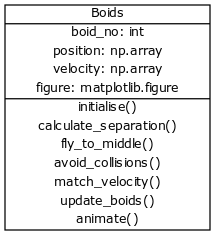
\includegraphics[width=0.7\textwidth]{UML.png}
   \captionof{figure}{UML diagram of the \texttt{Boids} class.}
   \label{fig:UML}
\end{Figure}



\section{Refactoring} \label{sec:Refactoring}
The refactoring approach has been based on material provided in the \href{http://development.rc.ucl.ac.uk/training/engineering/notes.pdf}{course lecture notes}. The initial code consisted of an inefficient algorithm with many magic numbers contained in one very large update function. This was gradually changed while still retaining the functionality of the code at each new commit. 
In the following section, we outline how the code was refactored and link to each commit where the change was performed. The full log of commits can be found \href{https://github.com/sqvarfort/bad-boids/commits/master}{here}.

 
\subsection{Identifying refactoring smells} 
The following smells were identified and corrected. 


\textit{Replacing magic numbers} This was done throughout the refactoring process, for example changing the number of Boids into an easily accessible variable \texttt{boid\_no}, \href{https://github.com/sqvarfort/bad-boids/commit/d0ecbd997414939af6c1769529e96ae970c5d931}{commit d0ecbd997414939af6c1769529e96ae970c5d931}. Also, \href{https://github.com/sqvarfort/bad-boids/commit/6b1c41966d0c6f48eced7ea55c872305b5c5f0ca}{commit  6b1c41966d0c6f48eced7ea55c872305b5c5f0ca} is another example of where we make sure the bounds of the graph adapt to the input values chosen by the user, instead of being defined as arbitrary numbers. 

\textit{Replacing repeated code with functions} Certain calculations, like working out the separation between all boids are required for more than one of the class methods. Therefore, these calculations have been placed in a separate method, \texttt{calculate\_separations()}, which is accessed once for each call of \texttt{update\_boids()}.  This makes each function more efficient. See \href{https://github.com/sqvarfort/bad-boids/commit/5119b660b00488bb33ab9dc246db279d8e020fef}{commit 5119b660b00488bb33ab9dc246db279d8e020fef} for these changes. 


\textit{Changing variable names} Variables and function names have been changed into a more readable format. The biggest change was when we replaced the iterated loops with \texttt{numpy} arrays in \href{https://github.com/sqvarfort/bad-boids/commit/d0ecbd997414939af6c1769529e96ae970c5d931}{commit d0ecbd997414939af6c1769529e96ae970c5d931}. 

\textit{Replacing loops with iterators} The greatest advantage brought to the new code is that of \texttt{numpy} which allows, through compact syntax, to carry out all the operations at once. This change was introduced early in \href{https://github.com/sqvarfort/bad-boids/commit/d0ecbd997414939af6c1769529e96ae970c5d931}{commit d0ecbd997414939af6c1769529e96ae970c5d931}. 

\textit{Replace constants with a configuration file} Similarly to replacing magic numbers, this was done in \href{https://github.com/sqvarfort/bad-boids/commit/db8654bb3b78cbf2aad4dc9b895bcb69f8704185}{commit db8654bb3b78cbf2aad4dc9b895bcb69f8704185}. 

\textit{Breaking up large functions} This was done in \href{https://github.com/sqvarfort/bad-boids/commit/267042203f6e372fc3af4206b46e16989d1301eb}{commit 267042203f6e372fc3af4206b46e16989d1301eb} where we split the \texttt{update\_boids()} method into several smaller methods. Each smaller method handled one instance of the flocking behaviour simulation. 

\textit{Separate code concepts into files or modules} Initially, the animation function was in the same file as the boid initialisation code. We moved the animation outside the class in a command-line interface file which calls the \texttt{Boids} class. See \href{https://github.com/sqvarfort/bad-boids/commit/979994280527631d6f5f0b41f8b2c14117ad24e0}{commit 979994280527631d6f5f0b41f8b2c14117ad24e0}. 


\section{Tests} \label{sec:Tests}
The original update function was divided into separate methods to make it more readable, but also in order to simplify testing. Three tests have been written for this implementations. 

Firstly, we have the regression test which ensures that the code functions correctly throughout the refactoring process. When changing the code structure to handle \texttt{numpy} arrays, the regression test was subsequently changed to interface with the new \texttt{Boids} class. Since the methods for velocity alteration perform the calculation in a different order, the regression test with an original tolerance of $\delta = 0.01$ fails. However, changing to $\delta = 0.06$ causes the test to pass, which indicates that the calculation stayed essentially the same. Since the change is very small, the regression test is deemed to still hold. In fact, rather than recording new fixtures, $\delta$ can be used as a measure of distance to the original code. 

Secondly, we have written tests for every method in the \texttt{Boids} class. Since the motion of many boids essentially constitutes an $N$-body problem, we have chosen to implement tests for interactions between a count of two boids. The motion of a two-body problem is predictable, and by choosing non-random initial positions and velocities, the effect of the various functions can be easily predicted. 

Finally, we have written tests for bad input to ensure that the code returns ValuError or TypeErrors when it encounters a problem, such as a negative number of boids or a non-existent configuration file. 




\section{Advantages of Refactoring} \label{sec:RefactoringAdvantages}
The most obvious advantage to refactoring the code is that the functionality of the code remains unchanged throughout the refactoring process. If a code is in continuous use, the refactoring can take place while still obtaining results from the code. Making sure that a regression test passes between every commit ensures that external uses can keep using the code.  However, changes to the code might cause small deviations in the calculations, as we saw for the methods in the \texttt{Boids} class. Whether this constitutes a problem depends on the nature of the calculation in question. 

The refactoring process also requires a good understanding of the original code. While this requires a time investment, it could also provide benefits in that the refactoring user can later utilise the code more efficiently. 



\section{Conclusions} \label{sec:Conclusion}
In this report, we have documented a refactoring process of a flocking behaviour simulation of so-called boids. We conclude that the refactoring approach is useful for maintaining the functionality of code while optimising it. Several code smells were identified and corrected through the refactoring progress. The final result is an efficient, readable and user-friendly packaged code. 


\end{multicols}



\iffalse

@inproceedings{reynolds1987flocks,
  title={Flocks, herds and schools: A distributed behavioral model},
  author={Reynolds, Craig W},
  booktitle={ACM SIGGRAPH computer graphics},
  volume={21},
  number={4},
  pages={25--34},
  year={1987},
  organization={ACM}
}

\fi
\end{document}